\documentclass[letterpaper,10pt]{article}
\usepackage[top=2cm, bottom=1.5cm, left=1cm, right=1cm]{geometry}
\usepackage{amsmath, amssymb, amsthm,graphicx}
\usepackage{fancyhdr}
\pagestyle{fancy}

\lhead{\today}
\chead{MATH 710 Assignment 8}
\rhead{Justin Hood}

\newcommand{\Z}{\mathbb{Z}}
\newcommand{\Q}{\mathbb{Q}}
\newcommand{\R}{\mathbb{R}}
\newcommand{\C}{\mathbb{C}}
\newtheorem{lem}{Lemma}

\begin{document}
\begin{enumerate}
\item Numerically solve the concentration (heat or diffusion) equation with homogeneous boundary conditions. Run the simulation up to a final time of $t_f=2$.
\begin{align*}
u_t &= \mu\frac{\partial^2 u}{\partial x^2},\ \ \ \ \mu\in(0,1] && (x,t)\in (0,1)\times (0,\infty) \\
u(0,t)&=0 && t\in (0,\infty)\\
u(1,t)&=0 && t\in (0,\infty)\\
u(x,0)&=\sin(\pi x) && x\in [0,1]
\end{align*}
We construct the matrix that defines the second spatial derivative using the CD2 stencil $L=\frac{1}{h^2}[1,-2,1]$. Then, we compute $u_{xx}=\mu*L\cdot u$ with a for loop over the interior of the $u$ matrix. We then apply the forward euler method to increment $u$ through time. We see that the equation behaves as we would expect, starting with a large peak of energy and diffusing down at the pace dictated by $\mu$. Below, we see the difference of two different $\mu$ as they are applied to the equation.
\begin{center}
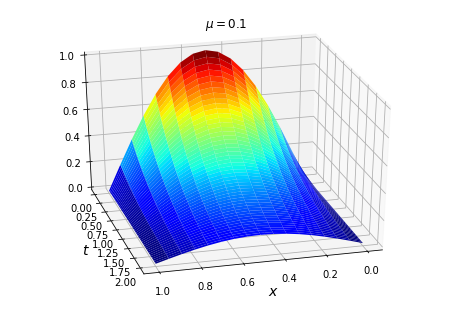
\includegraphics[scale=.8]{1mu1.png}
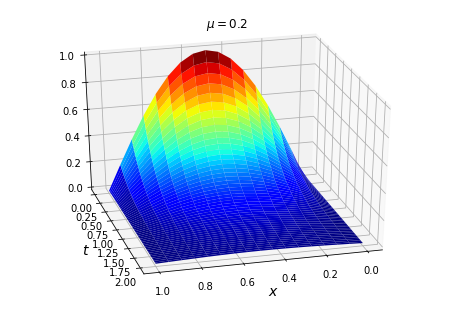
\includegraphics[scale=.8]{1mu2.png}
\end{center}
We see that as we increase $\mu$, the system diffuses faster, resulting in the steady state earlier.
\item See jupyter notebook.
\item We construct the second order accurate differentiation matrix with constant boundary conditions as seen below.
\[D=\begin{bmatrix}
1 & 0 & 0 & 0 & 0 & \ldots & 0 & 0 & 0 & 0\\
1 & -2 & 1 & 0 & 0 & \ldots & 0 & 0 & 0 & 0\\
0 & 1 & -2 & 1 & 0 & \ldots & 0 & 0 & 0 & 0\\
\vdots & & \ddots & \ddots & \ddots & \vdots & \vdots & \vdots & \vdots & \vdots\\
0 & 0 & 0 & 0 & 0 & \ldots & 1 & -2 & 1 & 0 \\
0 & 0 & 0 & 0 & 0 & \ldots & 0 & 1 & -2 & 1 \\
0 & 0 & 0 & 0 & 0 & \ldots & 0 & 0 & 0 & 1
\end{bmatrix}\]
Here, the first and last rows of the matrix represent the constant boundary conditions, and the interior rows represent the incremental derivatives $u_1',\ u_2',\ldots, u_{N-1}'$
\item Numerically solve Poisson's equation with homogeneous boundary conditions.
\begin{align*}
\frac{\partial ^2 u}{\partial x^2}&= && x\in (-1,1)\\
u(-1) &= 0\\
u(1) &= 0
\end{align*}
We may analytically solve this eqation,
\[u(x) = \sin(\pi x)\]
Thus, we may compare our solution numerically to the true solution to test accuracy. To numerically solve this equation, we write the equation in matrix form as,
\[Du=f,\ \ f=-\pi^2\sin(\pi x)\]
We then use \textit{numpy.linalg.solve} to compute the $u$ matrix. Finally, we plot the solution over the true solution for comparison.
\begin{center}
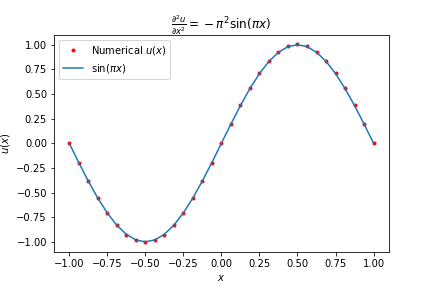
\includegraphics[scale=1]{4.png}
\end{center}
So, we see that the computed solution is accurate.
\item We now consider numerically solving the Poisson eqation defined as,
\begin{align*}
\frac{\partial^2 u}{\partial x^2}+\lambda u &= f(x) && x\in (-1,1)\\
u(-1) &= 0.808\\
u(1) &= 0.449
\end{align*}
We will attempt to solve the equation as before, considering now the Matrix equation,
\[Du+\lambda u=f(x)\Leftrightarrow (D+\lambda I)u = f(x)\]
Then, we use the \textit{linalg.solve} function to compute $u$. The result is as follows.
\begin{center}
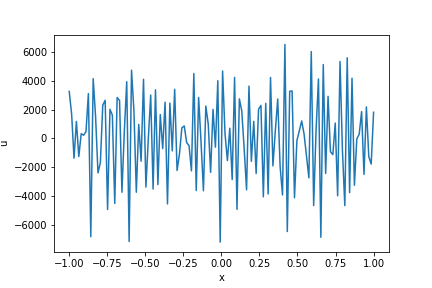
\includegraphics[scale=1]{5.png}
\end{center}
\item We solve Poisson's equation between two circular pipes. We assume the flow is steady and axisymmetric, i.e. $\frac{\partial w}{\partial \theta}=0$. Poisson's equation in polar coordinates is,
\[\nabla^2 w = \frac{G}{\mu} \Rightarrow \frac{1}{r}\frac{\partial}{\partial r}\bigg(\frac{\partial w}{\partial r}\bigg)+\frac{1}{r^2}\frac{\partial^2 w}{\partial \theta^2}=\frac{G}{\mu}\]
Based on our assumption, we can reduce this to,
\[\frac{1}{r}\frac{\partial}{\partial r}\bigg(\frac{\partial w}{\partial r}\bigg)=\frac{G}{\mu}\]
Let us now call $\frac{G}{\mu}=\eta$ and solve as,
\begin{align*}
\frac{1}{r}\frac{\partial}{\partial r}\bigg(\frac{\partial w}{\partial r}\bigg)&=\eta\\
&\Leftrightarrow\\
\frac{\partial}{\partial r}\bigg(\frac{\partial w}{\partial r}\bigg) &= \eta r
\end{align*}
Integrating with respect to $r$, we arrive at,
\[\frac{\partial w}{\partial r} = \frac{\eta r^2}{2}+c_1\]
Integrating again with respect to $r$, we arrive at,
\[w(r) = \frac{\eta r^3}{6}+c_1r+c_2\]
We now impose the boundary conditions,
\begin{align*}
\frac{\eta a^3}{6}+c_1 a+c_2 &= 0 && w(a)=0\\
\frac{\eta b^3}{6}+c_1 b+c_2 &= W && w(b)=W
\end{align*}
We now solve this system of equations in matrix form as,
\[\begin{bmatrix}
a & 1 \\
b & 1
\end{bmatrix}\begin{bmatrix}
c_1\\
c_2
\end{bmatrix}=\begin{bmatrix}
-\frac{\eta a^3}{6}\\
W-\frac{\eta b^3}{6}
\end{bmatrix} \]
Subtracting $R_1=R_1-R_2$ and $R_2=R_2-\frac{b}{a}R_1$
\[\left[ \begin{array}{cc|c}
a-b & 0 & -\frac{\eta a^3}{6}+\frac{\eta a^3}{6}-W\\
0 & 1-\frac{b}{a} & (W-\frac{\eta b^3}{6})+\frac{b}{a}\frac{\eta a^3}{6}
\end{array}\right]\]
Simplifying and solving,
\[c_1 =\frac{\eta}{6}\frac{b^3-a^3}{a-b}-\frac{W}{a-b}\]
\[c_2 = \frac{W}{1-\frac{b}{a}}+\frac{\eta}{6}\frac{ba^2-b^3}{1-\frac{b}{a}}\]
Thus, our final solution is,
\[w(r) = \frac{\eta r^3}{6}+\bigg(\frac{\eta}{6}\frac{b^3-a^3}{a-b}-\frac{W}{a-b}\bigg)r+\bigg(\frac{W}{1-\frac{b}{a}}+\frac{\eta}{6}\frac{ba^2-b^3}{1-\frac{b}{a}}\bigg)\]
\item We derive the Schwarzchild radius by the Laplacian method. First, we take the force equation and compute the squared velocity as follows.
\begin{align*}
m\frac{d^2r}{dt^2} &= -\frac{GMm}{r^2}\\
\frac{d}{dt}\frac{dr}{dt} &= -\frac{GM}{r^2}\\
\frac{d}{dt}v &= -GMr^{-2}\\
v &= -GM\int r^{-2} dt\\
v^2=v\frac{dr}{dt} &= -GM\int r^{-2} \frac{dr}{dt}dt=-GM\int r^{-2}dr\\
v^2 &= \frac{GM}{r}+C
\end{align*}
We now implement the initial condition $v(R)=v_e$ and solve for $C$.
\begin{align*}
v_e^2 &= \frac{GM}{R}+C\\
C&=v_e^2-\frac{GM}{R}
\end{align*}
So,
\[v^2=\frac{GM}{r}-\frac{GM}{R}+v_e^2\]
Next, we consider the limit as $r\to\infty$. Here, $v(r)\to 0$. Thus,
\[\lim_{r\to\infty} v(r)^2= \lim_{r\to\infty}\bigg[\frac{GM}{r}-\frac{GM}{R}+v_e^2\bigg]\Rightarrow 0=v_e^2-\frac{GM}{R}\Rightarrow v_e=\sqrt{\frac{GM}{R}}\]
We now set $v_e=c$, and solve for $R$
\[R_s=\frac{GM}{c^2}\]
We now compute the radii for various objects.\\
\begin{center}
\begin{tabular}{|r|l|l|}
\hline
$Object$ & $R_s$ & $Swarzchild\ radius$\\\hline \hline
$Sun (M=1.989\times 10^{30} kg)$ & $1476.923m$ & $2953.845m$ \\\hline
$Earth (M=5.972\times 10^{24}kg)$ & $0.0044m$ & $0.0089m$\\\hline
$Betelgeuse (M=2.387\times 10^{31}kg)$ & $17724.556$ & $35449.112$ \\\hline


\end{tabular}
\end{center}
\end{enumerate}
\end{document}
